
%(BEGIN_QUESTION)
% Copyright 2008, Tony R. Kuphaldt, released under the Creative Commons Attribution License (v 1.0)
% This means you may do almost anything with this work of mine, so long as you give me proper credit

In this time-delay relay circuit, the motor will immediately start when the pushbutton is pressed, and continue to run for about 5 seconds after the pushbutton is released.  The green light-emitting diode (LED) is supposed to be on whenever the motor is stopped, and off whenever the motor is running:

$$\includegraphics[width=15.5cm]{i03168x01.eps}$$

However, a problem has developed with this circuit.  Neither the motor nor the green LED ever energizes, no matter what is done with the pushbutton switch.  Strangely enough, the relay {\it does} make a ``click'' sound when the pushbutton is pressed, and then another ``click'' sound about 5 seconds after the switch is released.  Based on this information, determine the following:

\vskip 10pt

\begin{itemize}
\item{} \underbar{Two} components or wires in the circuit that you know cannot be failed either open or shorted, besides the 24 volt source.
\vskip 40pt
\item{} \underbar{Two} components or wires in the circuit you think could possibly be bad (either one independently capable of causing the problem), and the type of failure each would be (either open or shorted).
\end{itemize}

\vfil 

\underbar{file i03168}
\eject
%(END_QUESTION)





%(BEGIN_ANSWER)

This is a graded question -- no answers or hints given!

%(END_ANSWER)





%(BEGIN_NOTES)

\goodbreak
\noindent
{\bf Components known to be in good working condition:}

\begin{itemize}
\item{} Pushbutton switch
\item{} Capacitor
\item{} Relay coil
\end{itemize}

\vskip 10pt

\goodbreak
\noindent
{\bf Components which could possibly be faulted:}

\begin{itemize}
\item{} Wire from TP1 to TP4 broken (open)
\item{} Wire from TP4 to relay broken (open)
\item{} Wire from TP7 to TP8 broken (open)
\item{} Relay reed burnt so it cannot contact either ``throw''
\end{itemize}

%INDEX% Troubleshooting review: electric circuits

%(END_NOTES)


